\section{Algoritmo de aplanado}

\begin{frame}[fragile]
\frametitle{Algoritmo de aplanado} 
Está dividido en dos etapas:
\begin{block}{Reducción de composiciones}
\begin{enumerate}
\item Expansión de herencia.
\item Simplificación de tipos.
\item Aplicación de modificaciones.
\item Reducción de instancias. 
\end{enumerate}
\end{block}

\begin{block}{Resolución de conexiones}
Descomposición de ecuaciones \textit{connect} en ecuaciones de igualdad.
\end{block}
\end{frame}

\begin{frame}[fragile]
\frametitle{Algoritmo de aplanado} 
\begin{center}
\huge Reducción de composiciones
\end{center}
\end{frame}

\begin{frame}[fragile]
\frametitle{Algoritmo de Aplanado - Reducción de composiciones} 
\begin{lstlisting}[style=base,basicstyle=\scriptsize]
Flat(C):
    @2Expand(C);@
    foreach v in Variables(C):
        t = @2ResolveType(v)@;
        if isBasic(t) then 
            ChangeType(v,t);
        else if isClass(t) then
            @2ApplyModification(C,t,Modification(v));@
            Flat(t);
            @2RemoveComposition(C,t);@  
            if isConnector(t) then
                ChangeType(v,t);
            else
                Remove(t);
            end if;     
        end if;     
    end foreach;    
    foreach e in Equations(C):  
        @2ChangeVarName(e);@     
\end{lstlisting}
\end{frame}

\begin{frame}[fragile]
\frametitle{Expansión de herencias - Expand} 

\begin{block} {}
La clase hijo hereda las variables y ecuaciones del padre.
\end{block}

\pause 
\begin{columns} 
\column[t]{.5\textwidth}   
\begin{lstlisting}[style=base,basicstyle=\scriptsize]
model OnePort
    Pin p;
    Pin n;
    Real v;
    Real i;
equation
    v = p.v - n.v;
    i = p.i;
    i = -n.i;
end OnePort;
model Capacitor
    extends OnePort;
    parameter Real C = 1;
equation
    C * der(v) = i;
end Capacitor;
\end{lstlisting} 

\column[t]{.5\textwidth}  
\begin{lstlisting}[style=base,basicstyle=\scriptsize]
model Capacitor 
    @2Pin p;@
    @2Pin n;@
    @2Real v;@
    @2Real i;@
    parameter Real C = 1;
equation
    @2v = p.v - n.v;@
    @2i = p.i;@
    @2i = -n.i;@
    C * der(v) = i;
end Capacitor;
\end{lstlisting}
\end{columns}
\end{frame}


\begin{frame}[fragile]
\frametitle{Simplificación de tipos - ResolveType} 
\begin{columns} 
\column[t]{.5\textwidth}  
\begin{block}{}
Determina el tipo real de una variable y sus características: 
\begin{itemize}
    \item Prefijos de Tipos.
    \item Definición de Arreglos. 
    \item Presencia de modificaciones.
\end{itemize}
\end{block}
\column[t]{.5\textwidth}  
\pause
\begin{lstlisting}[style=base,literate={=}{$\leftarrow{}$}{1}{==}{$={}$}{1},escapechar=|,basicstyle=\scriptsize]
package Circuits
    @2model Capacitor@
        extends OnePort;
        parameter Real C == 1;
    equation
        C * der(v) == i;
    end Capacitor;
    
    model LC_circuit 
        @Capacitor cap(v(start == 1));@
        inductor ind(L == 2);
        Pin p1,p2,p3;
    equation
        ...
    end LC_circuit;
end Circuits    
\end{lstlisting}
\end{columns}
\end{frame}


\begin{frame}[fragile]
\frametitle{Aplicación de modificaciones - ApplyModification} 
\begin{block}{}
\begin{enumerate}
\item Expandir la clase.
\item Agregar las modificaciones a la variable correspondiente.
\end{enumerate}
\end{block}
\pause
Capacitor c (C=5,v(start=2))

\begin{columns} 
\column[t]{.5\textwidth}  
\begin{lstlisting}[style=base,basicstyle=\scriptsize]
model Capacitor 
    Pin p;
    Pin n;
    Real v;
    Real i;
    parameter Real C = 1;
equation
    v = p.v - n.v;
    i = p.i;
    i = -n.i;
    C * der(v) = i;
end Capacitor;
\end{lstlisting}
\pause
\column[t]{.5\textwidth}  
\begin{lstlisting}[style=base,basicstyle=\scriptsize]
model Capacitor 
    Pin p;
    Pin n;
    Real v @(start=2)@;
    Real i;
    parameter Real @C = 5@;
equation
    v = p.v - n.v;
    i = p.i;
    i = -n.i;
    C * der(v) = i;
end Capacitor;
\end{lstlisting}
\end{columns}
\end{frame}

\begin{frame}[fragile]
\frametitle{Reducción de instancias - RemoveComposition} 
\begin{block}{RemoveComposition}
\begin{enumerate}
\item Reemplaza las instancias de clases (previamente aplanadas).
\item Añade las variables y ecuaciones internas.
\item Renombrar las variables añadidas para evitar colisión de nombres.
\item Si la instancia está vectorizada: 
    \begin{enumerate}
    \item Agrega las variables vectorizadas.
    \item Encapsulamos las ecuaciones dentro de una ecuación \textit{for}.
    \end{enumerate} 
\end{enumerate}
\end{block}
\end{frame}

\begin{frame}[fragile,t]
\frametitle{RemoveComposition} 
\begin{block}{Variables}
\begin{enumerate}
\item Agrega un prefijo al nombre de las variables: "nombreInstancia\_".
\item Mantiene los prefijos de tipos y las definiciones de arreglos de las variables. 
\item Agrega una nueva dimensión si la instancia estaba vectorizada.   
\end{enumerate}
\end{block}
\pause
\begin{block}{Ecuaciones}
\begin{enumerate}
\item Renombra las variables que correspondan.
\item Reemplaza el operador ''.'' por guiones.
\item Encapsula las ecuaciones en un \textit{for} si la instancia está vectorizada.
\end{enumerate}
\end{block}
\end{frame}

\begin{frame}[fragile]
\frametitle{Algoritmo de Aplanado - Reducción de composiciones} 
\begin{lstlisting}[style=base,basicstyle=\scriptsize]
Flat(C):
    @2Expand(C);@
    foreach v in Variables(C):
        t = @2ResolveType(v)@;
        if isBasic(t) then 
            ChangeType(v,t);
        else if isClass(t) AND then
            @2ApplyModification(C,t,Modification(v));@
            Flat(t);
            @2RemoveComposition(C,t);@  
            if isConnector(t) then
                ChangeType(v,t);
            else
                Remove(t);
            end if;     
        end if;     
    end foreach;    
    foreach e in Equations(C):  
        @2ChangeVarName(e);@     
\end{lstlisting}
\end{frame}


\begin{frame}[fragile]
\frametitle{Reducción de composiciones: Ejemplo}
\begin{columns} 
\column[t]{7cm}  
\begin{lstlisting}[style=base,basicstyle=\scriptsize]
package Circuits
    model LC_circuit
        Pin p1,p2,p3;
    equation
        p1.v = p2.v;
        p2.v = p3.v;
    end LC_circuit;
    model LC_line
        constant Integer N = 10;
        LC_circuit lc[N];
        ground gr[N];
    equation
        connect(lc[N].p1,lc[N].p2)      
        for i in 1:N - 1 loop
            connect(lc[i + 1].p3,lc[i].p2);
        end for;
        for i in 1:N loop
            connect(gr.p[i],lc[i].p1);
        end for;
    end LC_line;
end Circuits;
\end{lstlisting}

\column[t]{7cm}  
\begin{figure}
      \centering
      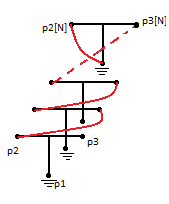
\includegraphics[scale=0.8]{lcline} 
    \end{figure}
\end{columns}
\end{frame}

\begin{frame}[fragile]
\frametitle{Reducción de composiciones: Ejemplo}
\begin{columns} 
\column[t]{7cm}  
\begin{lstlisting}[style=base,basicstyle=\scriptsize]
    @2model LC_circuit@
        Pin p1,p2,p3;
    equation
        p1.v = p2.v;
        p2.v = p3.v;
    end LC_circuit;
    
    model LC_line
        constant Integer N = 10;
        @2LC_circuit lc[N];@
        ground gr[N];
    equation
        connect(lc[N].p1,lc[N].p2)      
        for i in 1:N - 1 loop
            connect(lc[i + 1].p3,lc[i].p2);
        end for;
        for i in 1:N loop
            connect(gr.p[i],lc[i].p1);
        end for;
    end LC_line;
\end{lstlisting}
\pause
\column[t]{7cm}  
\begin{lstlisting}[style=base]
package Circuits
    model LC_circuit
        Pin p1,p2,p3;
        @flow Real p1_i,p2_i,p3_i;@
        @Real p1_v,p2_v,p3_v;@
    equation
        @p1_v = p2_v;@
        @p2_v = p3_v;@
    end LC_circuit;
end Circuits;
\end{lstlisting}
\end{columns}
\end{frame}

\begin{frame}[fragile]
\frametitle{Reducción de composiciones: Ejemplo}
\begin{columns} 
\column[t]{7cm}  
\begin{lstlisting}[style=base,basicstyle=\scriptsize]
    model LC_circuit
        Pin p1,p2,p3;
        flow Real p1_i,p2_i,p3_i;
        Real p1_v,p2_v,p3_v;
    equation
        p1_v = p2_v;
        p2_v = p3_v;
    end LC_circuit;
    
    model LC_line
        constant Integer N = 10;
        @2LC_circuit lc[N];@
        ground gr[N];
    equation
        connect(lc[N].p1,lc[N].p2)      
        for i in 1:N - 1 loop
            connect(lc[i + 1].p3,lc[i].p2);
        end for;
        for i in 1:N loop
            connect(gr.p[i],lc[i].p1);
        end for;
    end LC_line;
\end{lstlisting}
\pause
\column[t]{8cm}  
\begin{lstlisting}[style=base,basicstyle=\scriptsize]
package Circuits
    model LC_line
        constant Integer N = 10;
        Pin lc_p1[N], lc_p2[N], lc_p3[N];
        @flow Real lc_p1_i[N], lc_p2_i[N], lc_p3_i[N];@
        @Real lc_p1_v[N], lc_p2_v[N], lc_p3_v[N];@
        ground gr[N];
    equation
        @for i in 1:N loop@
            @lc_p1_v[N] = lc_p2_v[N];@
            @lc_p2_v[N] = lc_p3_v[N];@
        @end for;@
        connect(lc_p1[N],lc_p2[N])      
        for i in 1:N - 1 loop
            connect(lc_p3[i + 1],lc_p2[i]);
        end for;
        for i in 1:N loop
            connect(gr_p[i],lc_p1[i]);
        end for;
    end LC_line;
end Circuits;
\end{lstlisting}
\end{columns}
\end{frame}
